\chapter{Answer Candidate Type Selection}
\label{chap:candidate_generation}

% Comment: This chapter details your core methodological contribution for answer candidate generation

This chapter delves into specific methodologies developed to generate candidate answers by fusing the generative capabilities of Large Language Models (LLMs) with the structured factual knowledge encoded in Knowledge Graphs (KGs). As discussed in Chapter~\ref{chap:introduction}, while LLMs excel at text generation and comprehension, they often struggle with factual accuracy and are prone to generating plausible-sounding but incorrect information, a phenomenon often referred to as hallucination~\cite{lin-etal-2022-truthfulqa, DBLP:conf/emnlp/RobertsRS20}. Fusing LLMs with external KGs presents a compelling strategy to mitigate these limitations by grounding model outputs in verified factual structures~\cite{DBLP:journals/tkde/PanLWCWW24}. This integration process, broadly termed LLM-KG fusion, aims to leverage the strengths of both paradigms: the fluency and contextual understanding of LLMs (parametric knowledge) and the precision and reliability of KGs (non-parametric knowledge)~\cite{DBLP:conf/acl/MallenAZDKH23}.

Several approaches exist for this fusion. Some methods focus on encoding graph structure directly, using techniques like Graph Convolutional Networks (GCNs) for tasks like graph-to-text generation. However, recent work suggests that LLMs themselves, with appropriate prompting or fine-tuning, can often outperform specialized GCN architectures, particularly in handling the nuances of language and reducing factual errors~\cite{iarosh-etal-2025-reducing, DBLP:conf/ijcai/0001LW0S0Y24}. Another direction involves injecting knowledge more directly into the LLM parameters using techniques like adapters, attempting to distill relational facts into the model itself~\cite{DBLP:journals/corr/abs-2002-01808}. A prominent and flexible approach involves using the KG as an external knowledge source during inference, often retrieving relevant subgraphs or paths and incorporating this information into the LLM's prompt or generation process~\cite{DBLP:conf/emnlp/KnowledgeAugmented}.

This chapter focuses specifically on methods developed throughout our research that fall primarily within the category of generating high-quality answer candidates. We introduce the Answer Candidate Type (ACT) Selection~\cite{DBLP:journals/corr/abs-2310-07008} technique, which uses the LLM's understanding of semantic types combined with KG constraints to improve candidate generation. This method forms the foundation for the work detailed in the subsequent chapters, aiming to create more controllable and factually reliable QA systems.


\section{Answer Candidate Type Selection}
\label{sec:candidate_generation_type_selection}

While Large Language Models (LLMs) demonstrate impressive capabilities in various natural language tasks, their application to factoid Question Answering (QA) in a closed-book setting is often marred by factual inaccuracies and hallucinations \cite{DBLP:conf/emnlp/RobertsRS20, lin-etal-2022-truthfulqa}. Interestingly, however, even when an LLM fails to produce the correct factual answer, it often exhibits an understanding of the question's underlying intent and the semantic \textbf{type} of the expected answer. For instance, when asked "What is the official language of Brazil?", an LLM might incorrectly respond "Spanish" but correctly identify that the answer should be a \textbf{language}. Similarly, for "Who directed the movie Inception?", it might hallucinate a director's name but still understand the answer should be a \textbf{person} (specifically, a film director).

This observation suggests a potential avenue for improving factuality. If we can reliably predict the expected answer type, this information can serve as a valuable constraint. Knowing the type is particularly useful when combined with the main entity mentioned in the question. The correct answer entity within a Knowledge Graph (KG) is often located semantically "close" to the question entity, connected via specific relations, and, crucially, belongs to the expected semantic type. For example, knowing the question entity is "Brazil" and the answer type is `dbo:Language` significantly narrows down the plausible candidates within the KG compared to an unconstrained search or generation process.

This section presents our proposed approach, Answer Candidate Type~(ACT) Selection. We propose a universal approach to selecting the correct answer in the KGQA task by using any pre-trained large language model to generate answer candidates and to infer the type of expected answer. The answer candidate type selection pipeline shown in Figures~\ref{fig:act_selection:pipeline} and \ref{fig:act_selection:pipeline_example}.

\begin{figure}[]
    \centering
    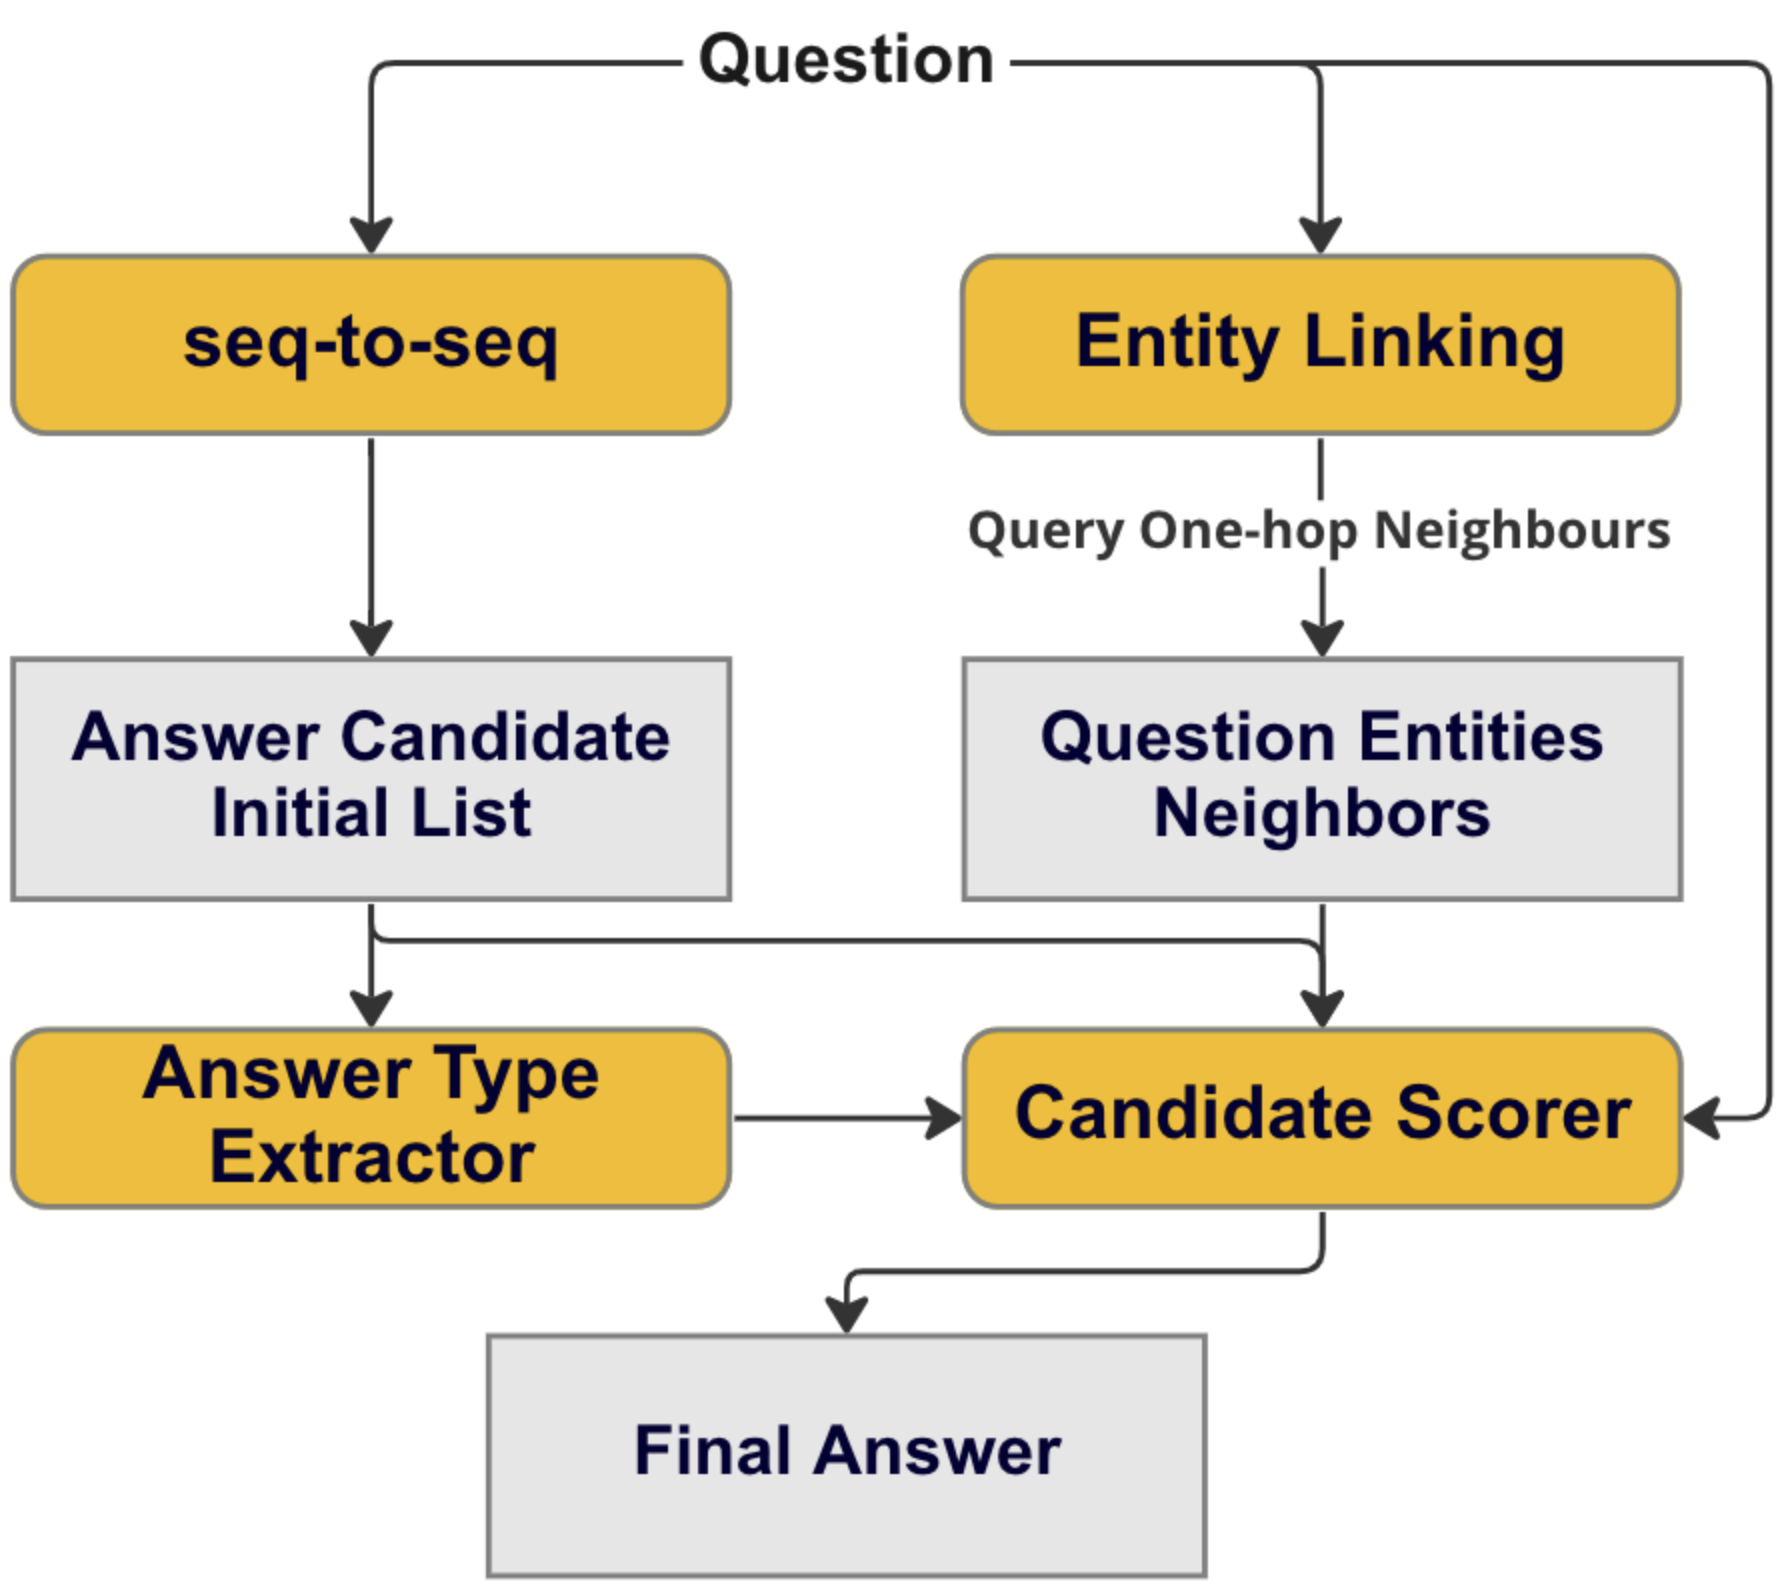
\includegraphics[width=0.85\textwidth]{act_selection/pipeline.png}
    \caption{ACT Selection Pipeline: (1) Put question to sequence to sequence language model to generate answer candidates, (2) Extract type from candidates, (3) Extract entities from the questions and query one-hop neighbors of the entities in the KG, (4) Filter candidates by type, (5) Select the best candidate.}
    \label{fig:act_selection:pipeline}
\end{figure}

\begin{figure}[]
    \centering
    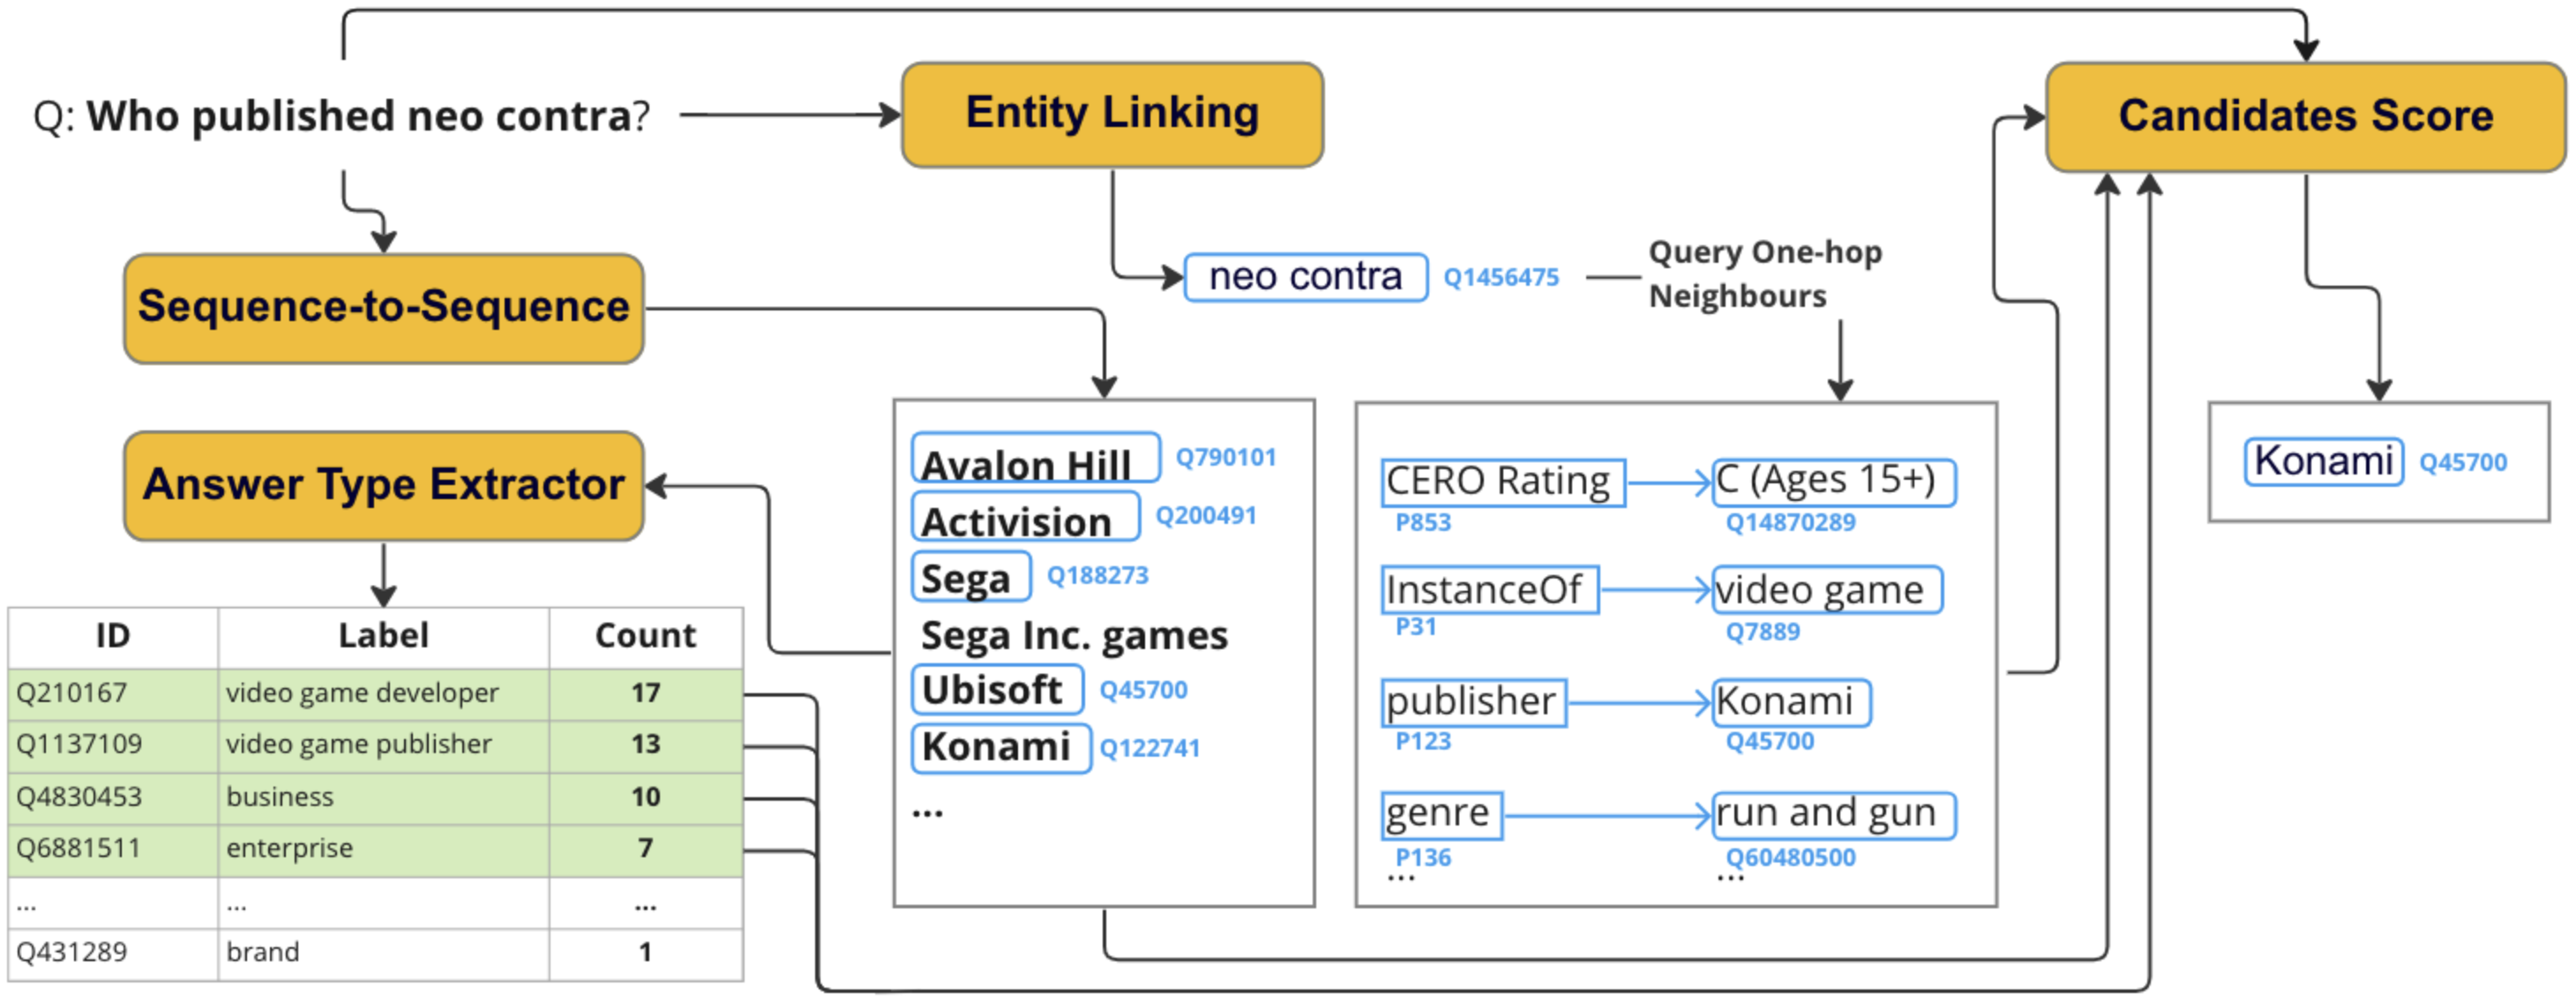
\includegraphics[width=0.95\textwidth]{act_selection/pipeline_example.png}
    \caption{The Answer Candidate Type (ACT) Selection pipeline for Knowledge Graph Question Answering (KGQA). The process combines a sequence-to-sequence model with knowledge graph-based entity linking and scoring to identify the correct answer, "Konami," as the publisher of "Neo Contra."}
    \label{fig:act_selection:pipeline_example}
\end{figure}

\section{Initial Answer Candidate Generation}
\label{sec:candidate_generation:initial_answer_candidate_generation}
When using \texttt{Classical Beam Search}, the output is often minor variations of a single sequence, which may not generate enough unique answer candidates for the Question Answering task. We use Diverse Beam Search~\cite{DBLP:journals/corr/VijayakumarCSSL16-diverse-beam-search} to generate an initial list of answer candidates.

The formula~\ref{eq:candidate_generation:diverse_beam_search} involves splitting the set of beams at time $t$ into $g$ disjointed subsets $Y_{[t]}^g$, and then selecting the candidate with the highest diversity penalty, which is calculated as the sum of a diversity penalty function $\Theta(y_{b,[t]}^g)$ over all candidates in the subset. Additionally, a dissimilarity term is included, which is calculated as the sum of a dissimilarity function $\Delta(y_{b,[t]}^g, Y_{[t]}^h)$ over all previous subsets $Y_{[t]}^h$ up to time $g-1$. The dissimilarity term is weighted by a parameter $\lambda_g$. This formula is used to optimize the selection of answer candidates in a computationally efficient manner.

\begin{equation}
    \begin{aligned}
        Y_{[t]}^g = \quad & \underset{y_1^{g}, \dots, y_{B\prime}^g \in Y_t^g} {\text{argmax}} \quad \underbrace{\sum_{b \in [B\prime]} \Theta(y_{b, [t]}^g)}_{\text{diversity penalty}} \\ 
        & + \underbrace{\sum_{h=1}^{g-1} \lambda_g \Delta(y_{b,[t]}^g, Y_{[t]}^h)}_{\text{dissimilarity term}},
    \end{aligned} 
    \label{eq:candidate_generation:diverse_beam_search}
\end{equation}

Using Diverse Beam Search instead of Greedy Search often leads to a better exploration of the search space by ensuring that alternative answers are considered.  We define the types of entities using the Wikidata property \texttt{instance\_of}~(P31). Note that an entity can be of multiple types. Finally, the initial list of answer candidates is used in the Answer Candidate Typing and the Candidate Scorer with the mined candidates. 

\subsection{Answer Candidate Typing} \label{act}
We rank all types by their frequency in the initial list of answer candidates. 
After that, we merge the top-$K$ most frequent types and similar types to the final list $T$.
Types similarity is calculated as cosine similarity between Sentence-BERT~\cite{reimers-2019-sentence-bert} embeddings of respective labels. The final types are defined as the ones where similarity is greater than a threshold.

A similar aggregation method using hypernyms (also known as ''is-a''  or ''instance-of'' relations) was used in the past to label clusters of words senses in distributional models~\cite{biemann2013text}: distributionally similar words share common hypernym and top common hypernyms are surprisingly good labels for sense clusters. The analogy in our method is that language models appear to produce a list of distributionally similar candidates.

\subsection{Entity Linking}
To enrich the list of candidates, we add all one-hop neighbors of the entities found in the question. For that, we use the fine-tuned spaCy Named Entity Recognition~(NER)\footnote{\url{https://spacy.io}.}

Based on a comprehensive review of state-of-the-art Named Entity Recognition (NER) systems \cite{vajjala-balasubramaniam-2022-really}, we evaluated the top three approaches: spaCy\footnote{\url{https://spacy.io}}, Stanza\footnote{\url{https://stanfordnlp.github.io/stanza/}}, and SparkNLP\footnote{\url{https://nlp.johnsnowlabs.com}}. Our analysis revealed that pre-trained NER models performed poorly on the Simple Question Wikidata (SQWD)~\cite{SQ_WD} dataset, with entity detection failure rates ranging from 64\% to 88\%. Among these systems, spaCy demonstrated the best performance, leading us to select its standard configuration\footnote{\url{https://spacy.io/usage/training/}} for further fine-tuning. The implementation of this pipeline required two critical pre-processing steps. First, we needed to identify the entity span to feed into the algorithm. This necessitated first extracting entity labels and their corresponding redirects, then locating these labels within the question text to determine spans. For entities without exact matches in the question, we employed fuzzy search techniques\footnote{\url{https://pypi.org/project/fuzzywuzzy/}}. Second, spaCy's training process requires entity type tags (e.g., PERSON for "Elon Musk", ORG for "Tesla" - following the BIO tagging scheme), which were not provided in the original datasets. We initially assigned the PERSON tag universally across all entities. Subsequent experiments with more precise entity type tagging did not yield significant improvements.
After extensive evaluation, we ultimately selected mGENRE \cite{decao2021multilingual} as our entity linking solution, which demonstrated superior performance compared to the NER-based approaches. mGENRE functions as an end-to-end entity linking system that eliminates the need for separate entity detection and disambiguation steps. Its multilingual autoregressive entity linking capabilities provided better accuracy and robustness across diverse question formulations in our experiments, making it a practical choice for our knowledge graph question answering pipeline.

\subsection{Candidates Scorer}
Finally, we calculate four scores for each entity from the answer candidate and rank them based on the weighted sum of the scores.
The scores are as follows:
% \begin{itemize}
    % \item
    \textbf{(1)~Type score} represents the size of the intersection between the set of types extracted from the answer candidates and the selected answer types. It is weighted by the number of selected answer types: $$S_\textrm{type}~=~\frac{|\textrm{Candidates' Types} \cap T|}{|T|}.$$

    % \item
\textbf{(2)~Forward one-hop neighbors score} $S_\textrm{neighbour}$ is  assigned 1 if the candidate is among the neighbors of the question entities, and 0 otherwise.

    % \item
\textbf{(3)~Text-to-Text answer candidate score} is determined by the rank of the candidate in the initial list $C$ generated by the Text-to-Text model divided by the size of the list: $$S_\textrm{t2t}~=~\frac{C.\textsc{}{index}(\textrm{Candidate})}{|C|}.$$

    % \item
\textbf{(4)~Question-Property Similarity score} $S_\textrm{property}$ measures the cosine similarity between the embeddings of the relevant property and the entire question. We employ Sentence-BERT~\cite{reimers-2019-sentence-bert} to encode the question, following a similar approach used for the Answer Candidate Type module.
% \end{itemize}
The four scores are calculated for each entity and then are combined to generate a final score that determines the entity's ranking. The answer with the highest weighted sum of scores in the candidate list is selected as the final answer:
%
$$S_\textrm{final} = S_\textrm{type} + S_\textrm{neighbour} + S_\textrm{t2t} + S_\textrm{property}.$$

\section{Experimental Design and Baselines}
\label{sec:candidate_generation_experimental_design}
% Comment: Describe the experimental setup used to evaluate the methods

\section{Results and Analysis: Demonstrating Factuality Improvements}
\label{sec:candidate_generation_results}
% Comment: Present the quantitative results comparing your methods against baselines.

\section{Chapter Summary}
\label{sec:candidate_generation_summary}
% Summary of answer candidate generation methods 